\chapter{Discussion}
\label{discussion}
\overridetextsize

\section{Low Resolution Images}

As shown in table \ref{tab:detection_results}, the detection performances on
CIFAR-10 are inferior compared to ImageNet or Dogs vs. Cats. I suppose that the
cause of this inferior result is that the perturbation needed to produce
adversarial examples on lower-resolution images (\emph{e.g.,} the ones from
CIFAR-10) is proportionally larger than on images with higher resolution.
Furthermore, as discussed in section \ref{sec:robustness}, more significant
adversarial perturbations are more robust to the random noise we add to the
images. Consequently, we need to use a larger $\kappa$ to improve the detection
for adversarial examples that contain a more significant relative adversarial
perturbation. However, while using a larger $\kappa$ proved to be helpful to
detect larger-perturbation adversarial examples, a $\kappa$ too high can
deteriorate normal images, leading the model not to recognize them, thus,
increasing the number of false positives.

\section{Adaptive Adversaries}

In all the experiments I presented, I considered adversaries who have full
access to the model parameters but do not adapt to bypass the detection method.
To do so, an adversary would need to produce examples such that both scores
remain under unknown thresholds, which is a considerably more challenging
problem than simply crafting adversarial examples. More challenging, primarily
because of the random nature of the technique, it would be extremely difficult
and time-consuming to generate adversarial examples that keep their adversarial
effects at varying unknown-to-the-adversary noise amounts.

Thus, it is highly challenging to generate adversarial examples that generalize
and keep their effect under all these \emph{unknown} and \emph{random}
parameters.

\clearpage
\section{Future Work}

\begin{figure}[!t]
    \subfloat[]{%
        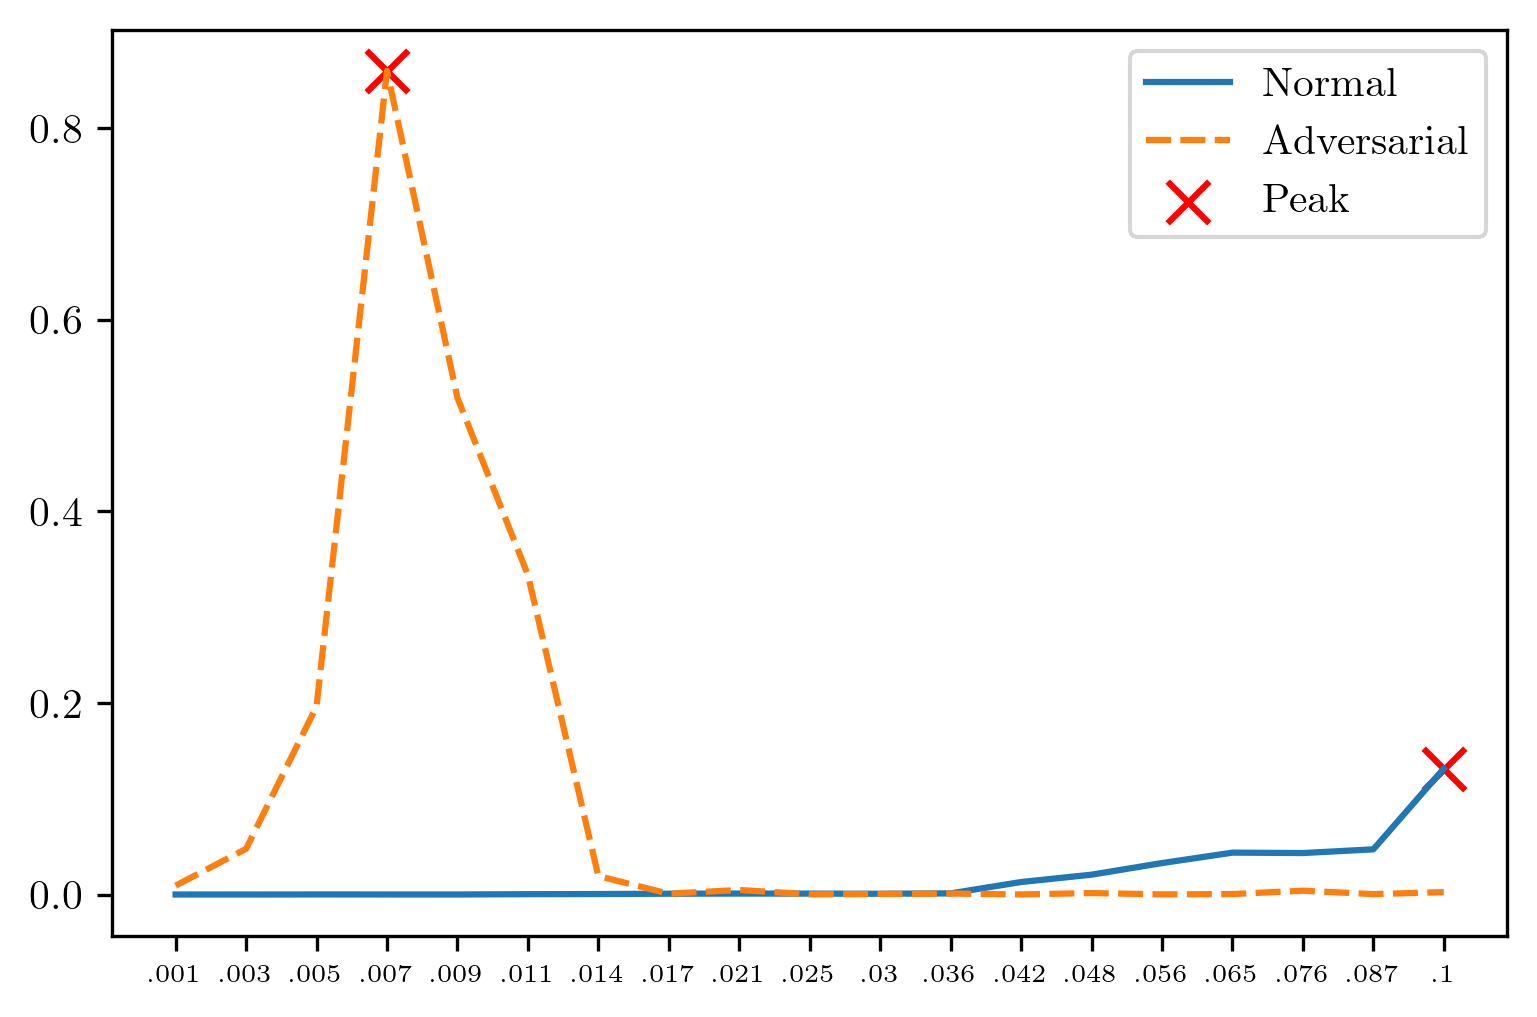
\includegraphics[clip,width=.5\linewidth]{Figures/peaks/1.png}%
    }
    \subfloat[]{%
        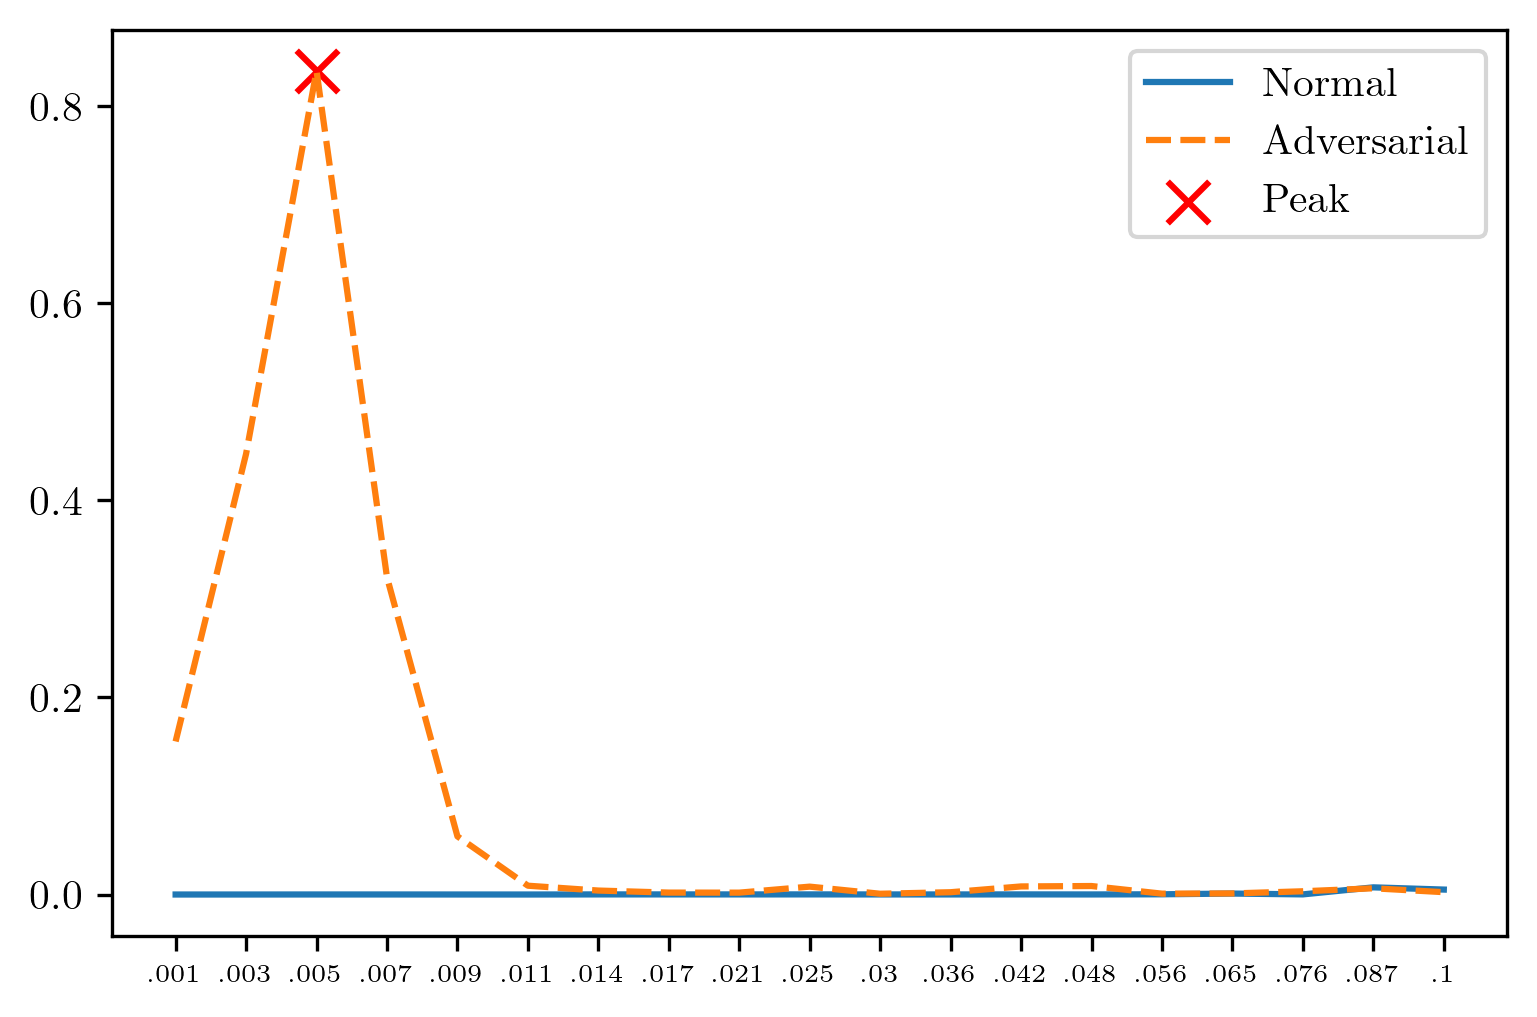
\includegraphics[clip,width=.5\linewidth]{Figures/peaks/3.png}%
    }

    \subfloat[]{%
        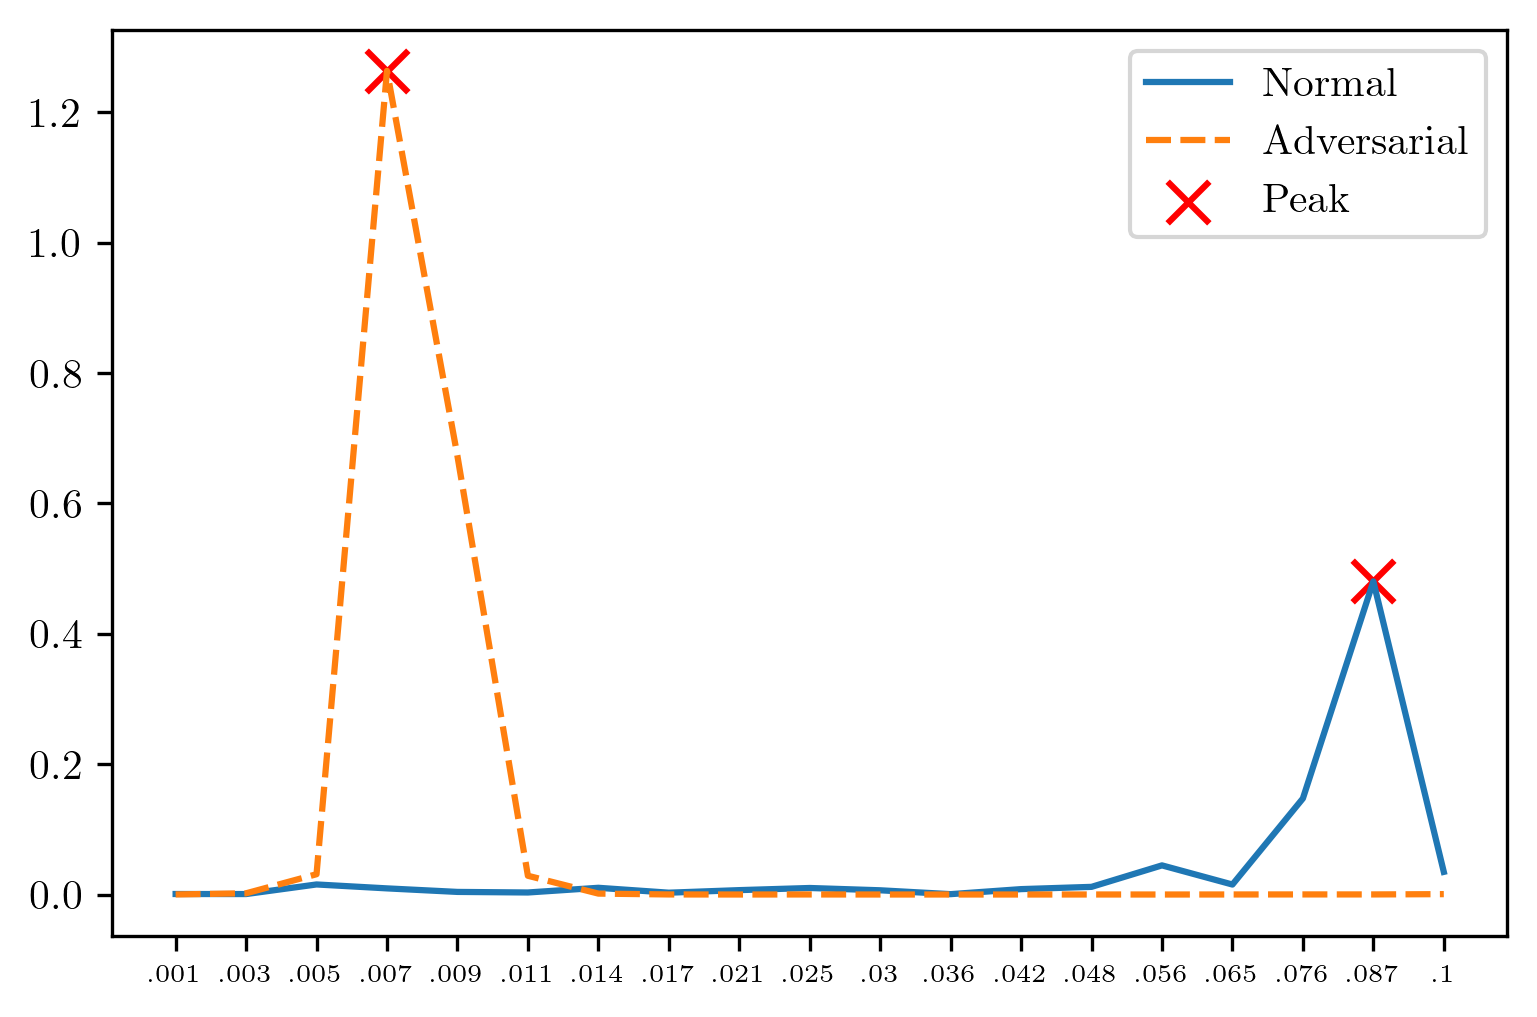
\includegraphics[clip,width=.5\linewidth]{Figures/peaks/13.png}%
    }
    \subfloat[]{%
        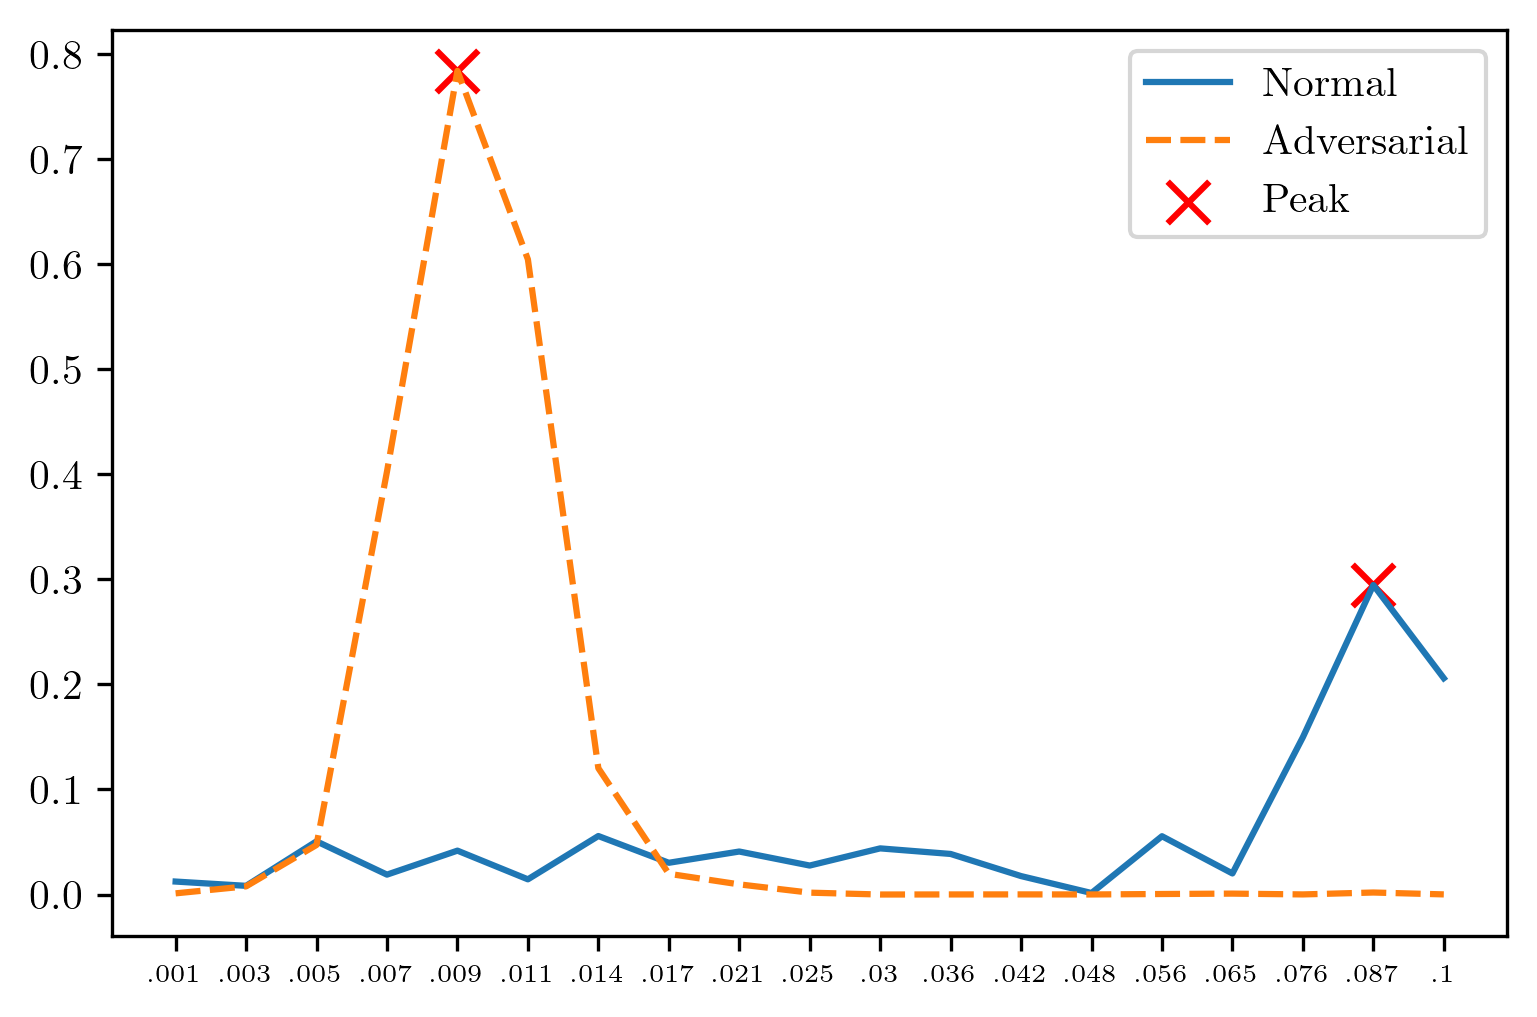
\includegraphics[clip,width=.5\linewidth]{Figures/peaks/20.png}%
    }

    \caption{Peaks observed on normal and adversarial images. Peaks on
        adversarial examples appear to happen at a sooner noise intensity and
        reach a higher value.}
    \label{fig:peaks}
\end{figure}
During my experiments, I wanted to explore different ways of detecting scores
anomalies. One of the ways I briefly experimented with was to plot the scores
differences at each noise intensity step. For example, given ten $\kappa$, I
computed the first-order difference like so:

\begin{align}
    \label{eq:first-order-diff}
    out_i= \lvert \alpha_{i+1} - \alpha_{i} \rvert,
\end{align}
where $\alpha_i$ represents the score result (either $score_1$ or $score_2$ seen
in \ref{eq:score1} and \ref{eq:score2}) at $\kappa_i$ noise intensity.

Figure \ref{fig:peaks} shows the plot of these score differences for four random
images and four adversarial examples generated with different methods. We
observe that the adversarial examples display high peaks earlier than normal
images. In most cases, normal images do not contain peaks at all. This
observation could be used to detect adversarial examples, \emph{e.g.,} by
comparing the intensity of the peaks and when they occur, \emph{i.e.,} when the
first-order difference peaks at an earlier $\kappa$, and at a high magnitude,
this could indicate the adversarial nature of the input.

Furthermore, for future research, I believe the detection performances of my
method could be improved by adding Gaussian noise as a form of data augmentation
during the training phase. Adding noise to the training data has been done
before to reduce overfitting or stabilize the models
\cite{zheng_improving_2016}. However, in combination with my method, I believe
that training the model with randomly modified inputs would improve the model's
robustness to noise and, thus, hypothetically reduce the number of false
positives, especially on lower resolution images like CIFAR-10, which increases
detection precision.